% =====================================================================
%  INFORME TÉCNICO · PRUEBA DE PENETRACIÓN
%  Proyecto de Hacking Ético · Módulo «Attacking Enterprise Networks» (HTB)
%  Archivo único. Compilar con pdfLaTeX (dos veces para el índice).
%  Sustituye el texto entre [corchetes] y añade tus capturas.
%  Diseño basado en la plantilla main.tex, adaptado a paleta ROJIZA.
%  Tipografía IBM Plex Sans / IBM Plex Mono · acento rojo #E5484D / #B01C22.
% =====================================================================
\documentclass[11pt,a4paper,oneside]{report}

% ---------------- Modo de color ----------------
% \oscurofalse: portada oscura e interior claro (recomendado para imprimir)
% \oscurotrue : todas las páginas con fondo oscuro, como la web
\newif\ifoscuro
\oscurofalse

% ---------------- Idioma y tipografía ----------------
\usepackage[T1]{fontenc}
\usepackage[utf8]{inputenc}
% Español de babel. En TeX Live completo / Overleaf se usa la definición nativa;
% si no está instalada (instalaciones mínimas), se carga desde el locale .ini.
\IfFileExists{spanish.ldf}
  {\usepackage[spanish,es-tabla]{babel}}
  {\usepackage[provide=*,main=spanish]{babel}}
\addto\captionsspanish{\renewcommand{\tablename}{Tabla}\renewcommand{\contentsname}{Índice}}
% IBM Plex Sans (texto y títulos) e IBM Plex Mono (etiquetas y números).
% Vienen con TeX Live completo y Overleaf; si no están, se usan Helvetica y Courier.
\IfFileExists{plex-sans.sty}
  {\usepackage[sfdefault]{plex-sans}}
  {\usepackage[scaled=0.92]{helvet}\renewcommand{\familydefault}{\sfdefault}}
\IfFileExists{plex-mono.sty}
  {\usepackage[scale=0.92]{plex-mono}}
  {\renewcommand{\ttdefault}{pcr}}
\usepackage{microtype}   % \textls{...}: espaciado entre letras de las etiquetas

% ---------------- Página ----------------
\usepackage[a4paper,top=2.8cm,bottom=2.6cm,left=2.8cm,right=2.8cm,headheight=18pt,headsep=14pt]{geometry}
\usepackage{setspace}
\usepackage{changepage}   % \begin{adjustwidth}{izq}{der} para el aviso legal
\setstretch{1.18}
\setlength{\parindent}{0pt}
\setlength{\parskip}{6pt plus 2pt}
\setlength{\emergencystretch}{1.6em}   % evita desbordes en párrafos con rutas/URL largas

% ---------------- Colores ----------------
\usepackage{xcolor}
% Paleta oscura (portada) con tinte cálido
\definecolor{negro}{HTML}{0A0607}       % fondo
\definecolor{puntos}{HTML}{1C1416}      % retícula de puntos
\definecolor{superficie}{HTML}{14100F}  % etiquetas y tarjetas
\definecolor{lineaweb}{HTML}{241A1B}    % líneas finas
\definecolor{bordeweb}{HTML}{3A2A2B}    % bordes
\definecolor{blanco}{HTML}{F4F2F2}      % texto principal
\definecolor{grisclaro}{HTML}{A49B9C}   % segunda línea del título
\definecolor{grismedio}{HTML}{968C8D}   % texto secundario
\definecolor{rojo}{HTML}{E5484D}        % acento sobre fondo oscuro
\definecolor{rojoboton}{HTML}{D1393E}   % botones
\definecolor{rojooscuro}{HTML}{B01C22}  % acento sobre fondo claro (más contraste)
% Colores de las páginas interiores según el modo
\ifoscuro
  \colorlet{fondo}{negro}
  \definecolor{tinta}{HTML}{EDE6E6}
  \colorlet{suave}{grisclaro}
  \colorlet{guia}{grismedio}
  \colorlet{acento}{rojo}
  \colorlet{borde}{bordeweb}
  \colorlet{zona}{superficie}
  \colorlet{filaalterna}{superficie}
  \colorlet{cabecera}{lineaweb}
  \colorlet{cabtexto}{blanco}
\else
  \colorlet{fondo}{white}
  \definecolor{tinta}{HTML}{1A1416}
  \definecolor{suave}{HTML}{6A5E60}
  \definecolor{guia}{HTML}{8A7E80}
  \colorlet{acento}{rojooscuro}
  \definecolor{borde}{HTML}{E6D9DA}
  \definecolor{zona}{HTML}{FBF4F4}
  \colorlet{filaalterna}{zona}
  \colorlet{cabecera}{negro}
  \colorlet{cabtexto}{white}
\fi
\color{tinta}            % color por defecto del texto
\ifoscuro\pagecolor{fondo}\fi

% Número con dos cifras (01, 02...); las letras de los anexos se dejan igual
\newcommand{\padnum}[1]{\ifnum0<0#1\relax\ifnum#1<10 0\fi\fi#1}
% Etiqueta: línea roja + texto monoespaciado espaciado
\newcommand{\etiqueta}[1]{{\color{acento}\rule[0.55ex]{1.1cm}{0.7pt}\hspace{0.35cm}%
  \ttfamily\small\textls[220]{\MakeUppercase{#1}}}}
% Esquina en escuadra
\newcommand{\esquina}{\hspace*{-0.55cm}\tikz{\draw[acento, line width=0.8pt]
  (0,0) -- (0,0.42) -- (0.42,0.42);}}
% Encabezado de capítulo: esquina + etiqueta
\newcommand{\rotulocap}[1]{\esquina\par\vspace{6pt}\etiqueta{#1}}

% ---------------- Títulos ----------------
\usepackage{titlesec}
\titleformat{\chapter}[display]
  {\normalfont\sffamily\color{tinta}}
  {\rotulocap{\chaptertitlename\ \padnum{\thechapter}}}
  {14pt}
  {\fontsize{28}{33}\selectfont\bfseries\raggedright}
  [\vspace{10pt}{\color{borde}\titlerule[0.6pt]}]
\titleformat{name=\chapter,numberless}[display]
  {\normalfont\sffamily\color{tinta}}
  {\rotulocap{Informe Técnico}}
  {14pt}
  {\fontsize{28}{33}\selectfont\bfseries\raggedright}
  [\vspace{10pt}{\color{borde}\titlerule[0.6pt]}]
\titlespacing*{\chapter}{0pt}{0pt}{22pt}
\titleformat{\section}{\normalfont\sffamily\Large\bfseries\color{tinta}\raggedright}
  {\ttfamily\mdseries\color{acento}\thesection}{0.8em}{}
\titleformat{\subsection}{\normalfont\sffamily\large\bfseries\color{tinta}\raggedright}
  {\ttfamily\mdseries\color{acento}\thesubsection}{0.8em}{}
\titlespacing*{\section}{0pt}{20pt plus 3pt}{6pt}
\titlespacing*{\subsection}{0pt}{14pt plus 2pt}{4pt}
\setcounter{secnumdepth}{2}
\setcounter{tocdepth}{2}

% ---------------- Índice ----------------
\usepackage{titletoc}
\titlecontents{chapter}[2.6em]{\addvspace{10pt}\sffamily\bfseries\color{tinta}}
  {\llap{\makebox[2.6em][l]{\ttfamily\mdseries\color{acento}\padnum{\thecontentslabel}}}}
  {}
  {\hfill\ttfamily\mdseries\color{suave}\thecontentspage}
\titlecontents{section}[5.6em]{\addvspace{1pt}\color{tinta}}
  {\llap{\makebox[3em][l]{\ttfamily\small\color{acento}\thecontentslabel}}}
  {}
  {\titlerule*[0.7pc]{\textcolor{borde}{.}}\ttfamily\small\color{suave}\thecontentspage}
\titlecontents{subsection}[8.8em]{\small\color{tinta}}
  {\llap{\makebox[3.2em][l]{\ttfamily\footnotesize\color{acento}\thecontentslabel}}}
  {}
  {\titlerule*[0.7pc]{\textcolor{borde}{.}}\ttfamily\footnotesize\color{suave}\thecontentspage}

% ---------------- Cabecera y pie ----------------
\usepackage{fancyhdr}
\pagestyle{fancy}
\fancyhf{}
\fancyhead[L]{{\ttfamily\scriptsize\color{suave}\textls[120]{\MakeUppercase{\leftmark}}}}
\fancyhead[R]{\ttfamily\scriptsize\color{acento}\textls[120]{PENTEST · INLANEFREIGHT}}
% Pie: número de página centrado entre dos líneas rojas
\newcommand{\barrapie}{{\color{acento}\rule[0.55ex]{0.8cm}{0.6pt}}}
\newcommand{\pie}{%
  \fancyfoot[C]{\barrapie\hspace{8pt}{\ttfamily\footnotesize\color{tinta}\padnum{\thepage}}\hspace{8pt}\barrapie}}
\pie
\renewcommand{\headrulewidth}{0.5pt}
\renewcommand{\headrule}{\ifdim\headrulewidth>0pt{\color{borde}\hrule height\headrulewidth width\headwidth}\fi}
\renewcommand{\chaptermark}[1]{\markboth{\thechapter.\ #1}{}}
\fancypagestyle{plain}{\fancyhf{}\pie\renewcommand{\headrulewidth}{0pt}}

% ---------------- Figuras, tablas y listas ----------------
\usepackage{graphicx}
\usepackage{float}   % [H]: la tabla se queda donde se escribe
\usepackage{caption}
\DeclareCaptionFont{etiq}{\ttfamily\color{acento}}
\DeclareCaptionLabelFormat{mayus}{\textls[120]{\MakeUppercase{#1}~#2}}
\captionsetup{font=small, labelfont={small,etiq}, labelformat=mayus, labelsep=quad}
\usepackage{enumitem}
\setlist{itemsep=2pt,topsep=4pt}
\setlist[itemize]{label=\textcolor{acento}{\rule[0.32ex]{4pt}{4pt}}}
\setlist[enumerate]{label=\textcolor{acento}{\ttfamily\small\padnum{\arabic*}}}
% Tablas con el contenido SIEMPRE centrado (horizontal y vertical)
\usepackage{array,tabularx,booktabs}
\renewcommand{\tabularxcolumn}[1]{m{#1}}
\newcolumntype{C}{>{\centering\arraybackslash}X}
\newcolumntype{K}{>{\hsize=0.62\hsize\centering\arraybackslash}X}
\newcolumntype{Y}{>{\hsize=1.38\hsize\centering\arraybackslash}X}
\newcolumntype{Q}{>{\hsize=0.75\hsize\centering\arraybackslash}X}
\newcolumntype{V}{>{\hsize=0.85\hsize\centering\arraybackslash}X}
\newcolumntype{Z}{>{\hsize=1.40\hsize\centering\arraybackslash}X}
\newcolumntype{P}[1]{>{\hsize=#1\hsize\centering\arraybackslash}X}
\usepackage{colortbl}
\renewcommand{\arraystretch}{1.35}

\newcommand{\estilotabla}[1][1.7]{%
  \setlength{\aboverulesep}{0pt}\setlength{\belowrulesep}{0pt}%
  \renewcommand{\arraystretch}{#1}}
\newcommand{\reglasup}{\noalign{{\color{acento}\hrule height 1.4pt}}}
\newcommand{\reglainf}{\noalign{{\color{tinta}\hrule height 0.8pt}}}
\newcommand{\cab}[1]{\textcolor{cabtexto}{\ttfamily\footnotesize\bfseries\textls[80]{\MakeUppercase{#1}}}}

% Etiquetas de severidad (color según el nivel)
\definecolor{sevcrit}{HTML}{8E1519}
\definecolor{sevalta}{HTML}{C2282D}
\definecolor{sevmedia}{HTML}{C9760E}
\definecolor{sevbaja}{HTML}{4B7A2B}
\newcommand{\sev}[2]{\colorbox{#1}{\textcolor{white}{\ttfamily\scriptsize\bfseries\,\textls[40]{\MakeUppercase{#2}}\,}}}
\newcommand{\scrit}{\sev{sevcrit}{Crítica}}
\newcommand{\salta}{\sev{sevalta}{Alta}}
\newcommand{\smedia}{\sev{sevmedia}{Media}}
\newcommand{\sbaja}{\sev{sevbaja}{Baja}}

% ---------------- Bloques de consola / comandos ----------------
\usepackage{listings}
\lstdefinestyle{consola}{%
  basicstyle=\ttfamily\scriptsize\color{tinta},
  backgroundcolor=\color{zona},
  frame=leftline, framerule=1.6pt, rulecolor=\color{acento},
  framexleftmargin=7pt, xleftmargin=9pt, xrightmargin=4pt,
  aboveskip=9pt, belowskip=9pt,
  breaklines=true, breakatwhitespace=false,
  breakindent=0pt, postbreak=\mbox{\textcolor{acento}{$\hookrightarrow$}\space},
  columns=fixed, basewidth=0.5em, keepspaces=true, showstringspaces=false,
  literate={á}{{\'a}}1 {é}{{\'e}}1 {í}{{\'i}}1 {ó}{{\'o}}1 {ú}{{\'u}}1
           {Á}{{\'A}}1 {É}{{\'E}}1 {ñ}{{\~n}}1 {Ñ}{{\~N}}1 {·}{{\textperiodcentered}}1
           {→}{{$\rightarrow$}}1 {←}{{$\leftarrow$}}1 {≈}{{$\approx$}}1
}
\lstnewenvironment{consola}{\lstset{style=consola}}{}

% ---------------- Diagrama ----------------
\usepackage{tikz}
\usetikzlibrary{positioning,fit,backgrounds,arrows.meta,calc,babel}

% ---------------- Enlaces ----------------
\usepackage[hidelinks]{hyperref}
\usepackage{xurl}

% ---------------- Huecos para imágenes ----------------
% \imagen{archivo}{pie de figura}{etiqueta}
\newcommand{\imagen}[3]{%
  \begin{figure}[H]
    \centering
    \IfFileExists{#1}%
      {\includegraphics[width=0.9\linewidth,height=0.42\textheight,keepaspectratio]{#1}}%
      {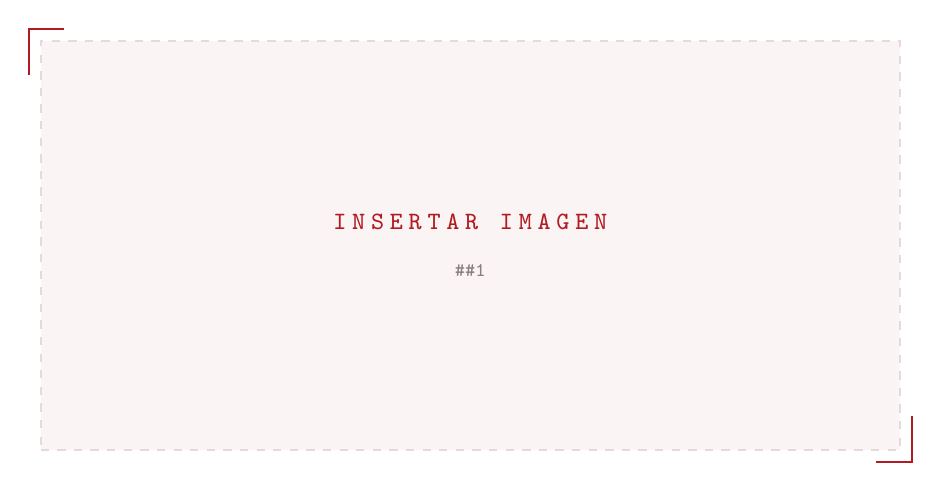
\begin{tikzpicture}
         \node[draw=borde, dashed, line width=0.6pt, fill=zona,
               minimum width=0.9\linewidth, minimum height=5.2cm, align=center] (h)
           {{\ttfamily\small\bfseries\color{acento}\textls[220]{INSERTAR IMAGEN}}\\[5pt]
            {\ttfamily\scriptsize\color{guia}\detokenize{#1}}};
         \draw[acento, line width=0.8pt] ($(h.north west)+(-4pt,-0.45cm)$) -- ++(0,0.45cm+4pt) -- ++(0.45cm,0);
         \draw[acento, line width=0.8pt] ($(h.south east)+(4pt,0.45cm)$) -- ++(0,-0.45cm-4pt) -- ++(-0.45cm,0);
       \end{tikzpicture}}%
    \caption{#2}\label{#3}%
  \end{figure}}

% Texto guía entre corchetes (en gris, para sustituir)
\newcommand{\guia}[1]{{\color{guia}\itshape[#1]}}

% =====================================================================
\begin{document}

% ============================ PORTADA ================================
\newcommand{\alumno}{Daniel Damota Maldonado}
\newcommand{\profesor}{Carlos Basulto Pardo}
\newcommand{\asignatura}{Hacking Ético}
\newcommand{\fechaentrega}{Noviembre de 2026}

\begin{titlepage}
\thispagestyle{empty}
\begin{tikzpicture}[remember picture, overlay,
    dato/.style={anchor=north west, inner sep=0pt, text width=7.2cm, align=left}]
\begin{scope}[shift={(current page.north west)}]
  % ---- Fondo y retícula de puntos ----
  \fill[negro] (-0.1,0.1) rectangle (21.1,-29.8);
  \foreach \x in {0.5,1.0,...,20.5}
    \foreach \y in {-0.5,-1.0,...,-29.5}
      \fill[puntos] (\x,\y) circle (0.4pt);
  % Arcos de fondo a la izquierda
  \draw[lineaweb, line width=0.5pt, dash pattern=on 1pt off 2pt] (-4,-15) circle (8.5);
  \draw[lineaweb, line width=0.5pt, dash pattern=on 1pt off 2pt] (-4,-15) circle (11);
  \draw[lineaweb, line width=0.5pt] (21.5,-2.5) circle (6.5);

  % ---- Redes de nodos (fondo) ----
  \tikzset{
    nodo/.pic={\fill[rojo] (0,0) circle (1.5pt);},
    nodohalo/.pic={\fill[rojo, opacity=0.16] (0,0) circle (8pt);
                   \draw[rojo, line width=0.6pt, opacity=0.8] (0,0) circle (4pt);
                   \fill[rojo] (0,0) circle (2pt);}}
  \coordinate (r1) at (8.0,-2.9);  \coordinate (r2) at (11.0,-0.7);
  \coordinate (r3) at (13.4,-2.4); \coordinate (r4) at (16.9,-1.4);
  \coordinate (r5) at (19.6,-3.1); \coordinate (r6) at (20.7,-0.5);
  \coordinate (r7) at (18.5,-5.7); \coordinate (r8) at (20.3,-8.6);
  \draw[rojo, line width=0.5pt, opacity=0.4]
    (r1) -- (r3) -- (r2)  (r3) -- (r4) -- (r5) -- (r6) -- (r4)
    (r5) -- (r7) -- (r8);
  \foreach \p in {r1,r2,r3,r5,r6,r7} \pic at (\p) {nodo};
  \foreach \p in {r4,r8} \pic at (\p) {nodohalo};
  \coordinate (s1) at (0.8,-19.0);  \coordinate (s2) at (4.2,-20.9);
  \coordinate (s3) at (7.9,-19.5);  \coordinate (s4) at (11.5,-21.4);
  \coordinate (s5) at (14.6,-19.1); \coordinate (s6) at (17.6,-21.0);
  \coordinate (s7) at (20.5,-18.4);
  \draw[rojo, line width=0.5pt, opacity=0.4]
    (s1) -- (s2) -- (s3) -- (s4) -- (s5) -- (s6) -- (s7)
    (s2) -- (s4)  (s3) -- (s5);
  \foreach \p in {s2,s3,s5,s6} \pic at (\p) {nodo};
  \foreach \p in {s1,s4,s7} \pic at (\p) {nodohalo};

  % ---- Esquinas en escuadra ----
  \draw[rojo, line width=0.7pt] (1.8,-3.9) -- (1.8,-3.3) -- (2.4,-3.3);
  \draw[rojo, line width=0.7pt] (19.2,-19.2) -- (19.2,-19.8) -- (18.6,-19.8);

  % ---- Etiqueta y título ----
  \draw[rojo, line width=0.7pt] (2.4,-4.2) -- (3.4,-4.2);
  \node[anchor=west, font=\ttfamily\small, text=rojo] at (3.7,-4.2)
    {\textls[280]{INFORME TÉCNICO · PRUEBA DE PENETRACIÓN}};
  \node[anchor=north west, inner sep=0pt, text width=17.2cm, align=left,
        font=\sffamily\bfseries\fontsize{34}{39}\selectfont, text=blanco] at (2.3,-4.95)
    {\textls[-30]{Attacking Enterprise}\\\textls[-30]{Networks}\\{\color{rojo}\textls[-30]{Informe técnico de pentesting}}};

  % ---- Párrafo ----
  \node[anchor=north west, inner sep=0pt, text width=8.4cm, align=left,
        font=\sffamily\fontsize{10.5}{16}\selectfont, text=grismedio] (parrafo) at (2.4,-11.9)
    {Prueba de penetración de alcance completo, en modalidad de caja negra, sobre la empresa
     ficticia \textcolor{blanco}{\bfseries Inlanefreight} del laboratorio autorizado de
     \textcolor{blanco}{\bfseries Hack The Box Academy}: desde el reconocimiento externo hasta
     el compromiso total del dominio de \textcolor{blanco}{\bfseries Active Directory}, con
     hallazgos valorados según CVSS~v4.0 y recomendaciones de remediación.};

  % ---- Botones ----
  \node[anchor=north west, fill=rojoboton, inner xsep=12pt, inner ysep=9pt,
        font=\sffamily\small\bfseries, text=white] (b1) at ([yshift=-0.9cm]parrafo.south west) {Informe técnico};
  \node[anchor=north west, draw=bordeweb, line width=0.6pt, fill=negro, inner xsep=12pt, inner ysep=9pt,
        font=\sffamily\small\bfseries, text=blanco] at ([xshift=0.3cm]b1.north east)
    {\tikz[baseline=-0.6ex]{\fill[rojo, rounded corners=0.8pt] (0,-0.1) rectangle (0.3,0.1);}\hspace{6pt}Inlanefreight · HTB CPTS};

  % ---- Emblema: objetivo/retícula sobre red empresarial + AD ----
  \begin{scope}[shift={(16.1,-13.9)}, scale=0.82]
    \coordinate (c) at (0,0);

    % Radar / órbitas de telemetría del objetivo
    \shade[inner color=rojo!30!negro, outer color=superficie] (c) circle (2.85);
    \draw[bordeweb, line width=0.5pt, dash pattern=on 0.8pt off 1.8pt] (c) circle (3.65);
    \draw[rojo, line width=0.45pt, opacity=0.6] (c) circle (3.2);
    \draw[rojo, line width=1.5pt] ([shift={(115:3.2)}]c) arc[start angle=115, end angle=215, radius=3.2];
    \draw[rojo, line width=1.5pt] ([shift={(-65:3.2)}]c) arc[start angle=-65, end angle=35, radius=3.2];

    % Ejes del punto de mira
    \begin{scope}[rojo, line width=0.65pt, opacity=0.85]
      \draw (0,2.1) -- (0,3.95);  \draw (0,-2.1) -- (0,-3.95);
      \draw (-2.1,0) -- (-3.95,0); \draw (2.1,0) -- (3.95,0);
    \end{scope}

    % Anillos del objetivo (retícula)
    \draw[rojo, line width=1.05pt] (c) circle (2.1);
    \draw[rojo, line width=0.7pt, opacity=0.75] (c) circle (1.45);
    \draw[rojo, line width=0.55pt, opacity=0.55] (c) circle (0.82);

    % Malla de red empresarial dentro del objetivo
    \begin{scope}
      \coordinate (n1) at (150:1.55); \coordinate (n2) at (90:1.05);
      \coordinate (n3) at (35:1.6);   \coordinate (n4) at (-40:1.5);
      \coordinate (n5) at (-110:1.3); \coordinate (n6) at (200:1.1);
      \draw[rojo, line width=0.5pt, opacity=0.8]
        (n1) -- (n2) -- (n3) -- (n4) -- (n5) -- (n6) -- (n1) (n2) -- (c) (n4) -- (c);
      \foreach \p in {n1,n2,n3,n4,n5,n6} \fill[blanco] (\p) circle (1.9pt);
      % Nodo central: controlador de dominio «en el punto de mira»
      \fill[rojo, opacity=0.28] (c) circle (9.5pt);
      \fill[rojo] (c) circle (4.4pt);
      \fill[blanco] (c) circle (1.7pt);
    \end{scope}

    % Etiquetas técnicas
    \node[font=\ttfamily\tiny\bfseries, text=rojo] at (0,1.72) {\textls[120]{RED · AD}};
    \node[fill=negro, draw=bordeweb, line width=0.5pt, rounded corners=1.5pt,
          inner xsep=5pt, inner ysep=2pt, font=\ttfamily\tiny\bfseries, text=blanco]
          at (0,-1.72) {\textls[140]{PENTEST}};
  \end{scope}

  % ---- Datos del trabajo ----
  \draw[lineaweb, line width=0.6pt] (2.4,-22.4) -- (18.6,-22.4);
  \node[dato] at (2.4,-23.05)
    {{\ttfamily\scriptsize\color{rojo}\textls[220]{ALUMNO}}\\[5pt]{\sffamily\color{blanco}\alumno}};
  \node[dato] at (10.8,-23.05)
    {{\ttfamily\scriptsize\color{rojo}\textls[220]{PROFESOR}}\\[5pt]{\sffamily\color{blanco}\profesor}};
  \node[dato] at (2.4,-24.85)
    {{\ttfamily\scriptsize\color{rojo}\textls[220]{MÓDULO}}\\[5pt]{\sffamily\color{blanco}\asignatura}};
  \node[dato] at (10.8,-24.85)
    {{\ttfamily\scriptsize\color{rojo}\textls[220]{FECHA DE ENTREGA}}\\[5pt]{\sffamily\color{blanco}\fechaentrega}};

  % ---- Pie ----
  \draw[lineaweb, line width=0.6pt] (-0.1,-27.9) -- (21.1,-27.9);
  \node[anchor=west, font=\ttfamily\tiny, text=grismedio] at (2.4,-28.55)
    {\textls[200]{CURSO DE ESPECIALIZACIÓN EN CIBERSEGURIDAD (CETI) · 2026--2027}};
  \node[anchor=east, font=\ttfamily\tiny, text=grismedio] at (18.6,-28.55)
    {\textls[200]{ENTORNO DE PRUEBAS AUTORIZADO · HTB}};
\end{scope}
\end{tikzpicture}
\end{titlepage}

% ============================ AVISO ÉTICO Y LEGAL ====================
\thispagestyle{empty}
\vspace*{3.5cm}
\begin{center}
{\ttfamily\small\color{acento}\textls[220]{AVISO ÉTICO Y LEGAL}}
\end{center}
\vspace{0.4cm}
\begin{adjustwidth}{1.2cm}{1.2cm}
\itshape
Todas las pruebas descritas en este documento se han realizado \textbf{exclusivamente} sobre el laboratorio del módulo \emph{Attacking Enterprise Networks} de Hack The Box Academy, un entorno de pruebas controlado y de uso \textbf{autorizado} por las condiciones del servicio. La empresa objetivo (\emph{Inlanefreight}), sus sistemas, sus usuarios y sus datos son \textbf{ficticios}. En ningún momento se ha dirigido actividad alguna contra sistemas reales, contra terceros conectados a la VPN ni contra la propia plataforma.

El acceso no autorizado a sistemas de información es un delito tipificado en el artículo~197~bis del Código Penal español. Este informe se elabora con fines estrictamente \textbf{académicos y defensivos}: su objetivo es documentar las debilidades encontradas y proponer su corrección. Las soluciones del laboratorio (respuestas, credenciales y \emph{flags}) no se publican; las credenciales y los datos sensibles aparecen \textbf{enmascarados} y se limitan a lo imprescindible para demostrar el impacto. El documento se entrega únicamente al profesorado del módulo.
\end{adjustwidth}
\clearpage

% ============================ ÍNDICE =================================
\pagenumbering{roman}
\begingroup
  \pagestyle{empty}
  \fancypagestyle{plain}{\fancyhf{}\renewcommand{\headrulewidth}{0pt}}
  \titleformat{name=\chapter,numberless}[block]
    {\normalfont\sffamily\color{tinta}}
    {}
    {0pt}
    {\fontsize{28}{33}\selectfont\bfseries\raggedright}
    [\vspace{10pt}{\color{borde}\titlerule[0.6pt]}]
  \tableofcontents
  \clearpage
\endgroup
\pagenumbering{arabic}

% ============================ 1 =====================================
\chapter{Resumen ejecutivo}

\section{Objeto del encargo}

Este documento recoge los resultados de una \textbf{prueba de penetración de alcance completo} realizada contra la red corporativa de la empresa ficticia \textbf{Inlanefreight}, correspondiente al módulo \emph{Attacking Enterprise Networks} de Hack The Box Academy, módulo final del itinerario \emph{Penetration Tester} que da acceso a la certificación \textbf{HTB~CPTS}. El encargo reproduce las condiciones de una auditoría real: una reunión de inicio (\emph{kickoff}), un alcance acordado, unas reglas de enfrentamiento y un plazo de pruebas definido.

La prueba se abordó desde la perspectiva de un \textbf{atacante externo anónimo} de Internet (caja negra), sin credenciales ni información interna previa. El único punto de entrada era un servidor perimetral expuesto; una vez comprometido, la prueba continuó hacia la red interna hasta alcanzar el dominio de Active Directory \texttt{INLANEFREIGHT.LOCAL}. El presente informe constituye el entregable \emph{informe técnico}, y detalla paso a paso la metodología, la cadena de ataque, los hallazgos y su remediación.

\section{Resultado global}

El resultado del encargo es \textbf{concluyente}: partiendo de cero información y desde el exterior, se consiguió \textbf{el compromiso total del dominio}, obteniendo privilegios equivalentes a los de un administrador de dominio (\emph{Domain Admin}). Ningún hallazgo aislado fue, por sí solo, determinante; como es habitual en los compromisos graves, el impacto fue el resultado de \textbf{encadenar debilidades} aparentemente menores —un servicio mal configurado, una aplicación web desactualizada y la reutilización de credenciales— hasta alcanzar los activos más valiosos de la organización.

La cadena de ataque siguió, de forma resumida, estas etapas:
\begin{enumerate}
  \item Reconocimiento externo y enumeración de la superficie expuesta (hosts, puertos, servicios y subdominios de \texttt{inlanefreight.local}).
  \item Explotación de una o varias aplicaciones web del perímetro para obtener un acceso inicial al servidor expuesto (DMZ).
  \item Escalada de privilegios local y establecimiento de un acceso estable, controlado y reversible.
  \item \emph{Pivoting} hacia las redes internas (\texttt{172.16.8.0/23} y \texttt{172.16.9.0/23}), no accesibles directamente desde Internet.
  \item Enumeración de Active Directory, ataques a credenciales de dominio y movimiento lateral.
  \item Compromiso del controlador de dominio y evaluación del impacto sobre los datos de la organización.
\end{enumerate}

\section{Panorama de severidad}

La Tabla~\ref{tab:resumen-sev} resume los hallazgos por nivel de severidad, valorados con \textbf{CVSS~v4.0} y ajustados según la exposición real del activo y su papel en la cadena de ataque. El detalle de cada hallazgo se desarrolla en el capítulo~\ref{cap:hallazgos}.

\begin{table}[H]
  \centering
  \caption{Resumen de hallazgos por severidad}
  \label{tab:resumen-sev}
  \small
  \estilotabla
  \begin{tabularx}{\linewidth}{P{1.8} P{0.8} P{0.8} P{0.8} P{0.8}}
    \reglasup
    \rowcolor{cabecera}
    \cab{} & \cab{Crítica} & \cab{Alta} & \cab{Media} & \cab{Baja} \\
    \rowcolor{filaalterna}
    \textbf{N.º de hallazgos} & \guia{n} & \guia{n} & \guia{n} & \guia{n} \\
    \reglainf
  \end{tabularx}
\end{table}

\guia{Ajusta los recuentos con tus hallazgos reales una vez completes el capítulo 4. Como referencia, un recorrido típico de este módulo arroja del orden de 2--3 hallazgos críticos (acceso inicial y compromiso de dominio), 4--6 altos (credenciales y AD), varios medios y alguno bajo.}

\section{Impacto para el negocio}

Trasladado a una organización real como la que representa Inlanefreight, el compromiso demostrado permitiría a un atacante: cifrar o destruir la información de toda la compañía (escenario de \emph{ransomware}), acceder a datos personales de empleados y clientes —con las consiguientes obligaciones de notificación de brechas—, suplantar a cualquier usuario o servicio del dominio y mantener la persistencia de forma prolongada. En términos prácticos, el nivel de acceso alcanzado equivale al \textbf{control efectivo de toda la infraestructura} basada en Active Directory.

\section{Recomendaciones principales}

Las medidas prioritarias, desarrolladas en la sección~\ref{sec:recomendaciones}, son:
\begin{itemize}
  \item \textbf{Reducir la superficie externa}: exponer solo los servicios imprescindibles, mantenerlos actualizados y retirar la información técnica innecesaria (versiones, mensajes de error, transferencias de zona DNS).
  \item \textbf{Robustecer las aplicaciones web}: validar entradas, corregir las inyecciones y la subida de ficheros, y aplicar el principio de mínimo privilegio en las cuentas de servicio.
  \item \textbf{Segmentar la red}: impedir que un servidor de la DMZ alcance libremente la red interna y el dominio.
  \item \textbf{Fortalecer Active Directory}: contraseñas robustas para las cuentas de servicio (frente a \emph{Kerberoasting}), revisión de ACL y privilegios excesivos, y protección de las credenciales en memoria y en recursos compartidos.
\end{itemize}

% ============================ 2 =====================================
\chapter{Alcance, reglas y metodología}

\section{Alcance del encargo}

El alcance se corresponde con el definido en el anteproyecto y en las reglas del escenario del módulo. La Tabla~\ref{tab:alcance} resume qué entra y qué queda fuera de la prueba.

\begin{table}[H]
  \centering
  \caption{Alcance de la prueba de penetración}
  \label{tab:alcance}
  \footnotesize
  \estilotabla[1.5]
  \begin{tabularx}{\linewidth}{P{1.0} P{1.0}}
    \reglasup
    \rowcolor{cabecera}
    \cab{Incluido en el alcance} & \cab{Fuera del alcance} \\
    \rowcolor{filaalterna}
    Laboratorio completo del módulo \emph{Attacking Enterprise Networks}. & Ingeniería social, \emph{phishing} y ataques físicos (excluidos por las reglas del escenario). \\
    Prueba externa del host expuesto y de los subdominios de \texttt{inlanefreight.local}. & Acciones destructivas o de denegación de servicio (DoS). \\
    \rowcolor{filaalterna}
    Continuación interna tras comprometer la DMZ: redes \texttt{172.16.8.0/23} y \texttt{172.16.9.0/23}. & Cambios en el entorno no autorizados por escrito por el cliente ficticio. \\
    Ataques al dominio \texttt{INLANEFREIGHT.LOCAL} hasta su compromiso total. & Evasión de antivirus o EDR: el escenario no la exige. \\
    \rowcolor{filaalterna}
    Persistencia controlada, documentada y revertida al cierre. & Redes inalámbricas, no incluidas en el laboratorio. \\
    Dos pasadas: una guiada y otra autónoma. & Cualquier sistema real o ajeno al laboratorio, incluida la plataforma de Hack The Box. \\
    \reglainf
  \end{tabularx}
\end{table}

\section{Reglas de enfrentamiento}

Las reglas de enfrentamiento fijan el marco del encargo y se tratan como un contrato con el cliente (Tabla~\ref{tab:roe}). Antes de cada fase se comprobó que la actividad prevista las cumplía.

\begin{table}[H]
  \centering
  \caption{Reglas de enfrentamiento del escenario}
  \label{tab:roe}
  \footnotesize
  \estilotabla[1.5]
  \begin{tabularx}{\linewidth}{P{0.85} P{1.15} P{1.0}}
    \reglasup
    \rowcolor{cabecera}
    \cab{Aspecto} & \cab{Condición del escenario} & \cab{Implicación para la prueba} \\
    \rowcolor{filaalterna}
    \textbf{Tipo de prueba} & Externa de alcance completo, desde un usuario anónimo de Internet, sin evasión. & Caja negra: no se parte de información interna. \\
    \textbf{Continuación interna} & Si se compromete la DMZ, la prueba continúa hacia Active Directory. & El \emph{pivoting} y los ataques al dominio están autorizados. \\
    \rowcolor{filaalterna}
    \textbf{Credenciales} & No se facilitan credenciales de aplicaciones, VPN ni Active Directory. & Todo acceso debe obtenerse durante la prueba. \\
    \textbf{Escaneos} & Permitidos siempre que no interrumpan los servicios; los intensivos, después de las 18:00 (hora de Londres). & Control del ritmo y planificación horaria de los escaneos. \\
    \rowcolor{filaalterna}
    \textbf{Ventana de pruebas} & Autorizada 24/7. & Flexibilidad para organizar las sesiones. \\
    \textbf{Actividades prohibidas} & \emph{Phishing}, ingeniería social, ataques físicos, DoS y cambios sin consentimiento escrito. & Toda modificación se registra y se revierte al cierre. \\
    \reglainf
  \end{tabularx}
\end{table}

\section{Entorno y equipo auditor}

La prueba se lanzó desde una máquina virtual con \textbf{Kali Linux} conectada al laboratorio mediante un túnel \textbf{OpenVPN}; como alternativa de respaldo se contempló \emph{Pwnbox}. La Tabla~\ref{tab:activos} recoge los activos del alcance y el entorno del equipo auditor, y la Figura~\ref{fig:entorno} muestra la topología lógica del laboratorio y las fases de la prueba.

\begin{table}[H]
  \centering
  \caption{Activos del alcance y equipo auditor}
  \label{tab:activos}
  \footnotesize
  \estilotabla[1.45]
  \begin{tabularx}{\linewidth}{P{0.9} P{0.9} P{1.1} P{1.1}}
    \reglasup
    \rowcolor{cabecera}
    \cab{Elemento} & \cab{Función} & \cab{Tecnología / servicios} & \cab{Direccionamiento} \\
    \rowcolor{filaalterna}
    \textbf{Equipo auditor} & Origen de todas las pruebas & Kali Linux (VM local) & Interfaz \texttt{tun0} (VPN) \\
    \textbf{Pwnbox} & Respaldo si falla la VPN & Máquina de ataque de HTB & Asignada por la plataforma \\
    \rowcolor{filaalterna}
    \textbf{Servidor perimetral (DMZ)} & Objetivo externo y punto de pivote & FTP, SSH, correo, DNS y web & \texttt{10.129.x.x} · interfaz interna en \texttt{172.16.8.0/23} \\
    \textbf{Aplicaciones web} & Superficie web externa & Subdominios \texttt{*.inlanefreight.local} & Resolución local en \texttt{/etc/hosts} \\
    \rowcolor{filaalterna}
    \textbf{Red interna} & Servidores y equipos del dominio & Hosts Windows y Linux & \texttt{172.16.8.0/23} y \texttt{172.16.9.0/23} \\
    \textbf{Dominio AD} & Objetivo final & \texttt{INLANEFREIGHT.LOCAL} & Controlador de dominio en la red interna \\
    \reglainf
  \end{tabularx}
\end{table}

\begin{figure}[H]
\centering
\resizebox{\linewidth}{!}{%
\begin{tikzpicture}[
    font=\sffamily\scriptsize,
    equipo/.style={draw=tinta!70, line width=0.7pt, fill=fondo, rounded corners=2pt,
                   text width=3.9cm, minimum height=1.9cm, align=center, inner sep=4pt},
    objetivo/.style={draw=acento, line width=1pt, fill=zona, rounded corners=2pt,
                   text width=3.9cm, minimum height=1.9cm, align=center, inner sep=4pt},
    zona/.style={draw=borde, line width=0.6pt, fill=zona, rounded corners=4pt, inner sep=9pt},
    rotulo/.style={font=\sffamily\scriptsize\bfseries, text=acento, align=center},
    flujo/.style={draw=acento, line width=1pt, -{Stealth[length=2.6mm]}},
    etiq/.style={fill=fondo, draw=acento, line width=0.6pt, rounded corners=2pt,
                 inner xsep=4pt, inner ysep=2pt, align=center, font=\sffamily\tiny, text=acento}
  ]
  % --- Equipo auditor (alineado con el centro vertical de las zonas) ---
  \node[equipo] (kali) at (0,-0.5)
    {\textbf{Equipo auditor}\\[2pt]Kali Linux\\[2pt]{\tiny nmap · Burp · BloodHound · Impacket}};

  % --- Zona DMZ ---
  \node[objetivo] (dmz) at (6.1,0.75)
    {\textbf{Servidor perimetral}\\[1pt]DMZ · \texttt{10.129.x.x}\\[2pt]{\tiny FTP · SSH · SMTP/POP3\\[1pt]DNS · HTTP/S}};
  \node[equipo] (web) at (6.1,-1.85)
    {\textbf{Aplicaciones web}\\[1pt]\texttt{*.inlanefreight.local}\\[2pt]{\tiny vhosts · subdominios}};

  % --- Zona interna ---
  \node[equipo] (int) at (13.2,0.75)
    {\textbf{Servidores y equipos}\\[2pt]{\ttfamily\tiny 172.16.8.0/23\\[1pt]172.16.9.0/23}\\[2pt]{\tiny SMB · RDP · WinRM · LDAP}};
  \node[objetivo] (dc) at (13.2,-1.85)
    {\textbf{Controlador de dominio}\\[1pt]\texttt{INLANEFREIGHT.LOCAL}\\[2pt]{\tiny objetivo final · Domain Admins}};

  % --- Zonas (al fondo) ---
  \begin{scope}[on background layer]
    \node[zona, fit=(dmz)(web), label={[rotulo, anchor=south]north:PERÍMETRO EXTERNO · DMZ}] (zdmz) {};
    \node[zona, fit=(int)(dc), label={[rotulo, anchor=south]north:RED INTERNA · ACTIVE DIRECTORY}] (zint) {};
  \end{scope}

  % --- Flujos entre zonas, con etiqueta en caja sobre la flecha ---
  \draw[flujo] (kali.east) -- (zdmz.west);
  \node[etiq] at ($(kali.east)!0.5!(zdmz.west)$) {OpenVPN};

  \draw[flujo] (zdmz.east) -- (zint.west);
  \node[etiq] at ($(zdmz.east)!0.5!(zint.west)$) {\textbf{pivoting}\\Ligolo-ng · Chisel};

  % --- Flujo interno hacia el controlador de dominio ---
  \draw[flujo] (int.south) -- (dc.north);

  % --- Fases ---
  \node[draw=borde, fill=fondo, rounded corners=2pt, anchor=north, text width=15.6cm,
        align=left, font=\sffamily\tiny, inner sep=6pt] at ($(zdmz.south)!0.5!(zint.south)+(0,-0.7)$)
    {\textbf{\color{acento}Fases de la prueba:}\quad
     1. Reconocimiento y explotación externa~~·~~2. Acceso inicial y persistencia en la DMZ~~·~~
     3. Pivoting y reconocimiento interno~~·~~4. Escalada y movimiento lateral~~·~~
     5. Compromiso de Active Directory~~·~~6. Post-explotación, cierre e informe.};
\end{tikzpicture}}
\caption{Topología lógica del laboratorio, segmentos y fases de la prueba}
\label{fig:entorno}
\end{figure}

\section{Metodología}

La prueba sigue las fases del \textbf{Penetration Testing Execution Standard (PTES)} y las recomendaciones de la guía \textbf{NIST SP~800-115}. Las aplicaciones web se evalúan con la \textbf{OWASP Web Security Testing Guide (WSTG)}, cada técnica se relaciona con \textbf{MITRE ATT\&CK} y cada vulnerabilidad confirmada se valora con \textbf{CVSS~v4.0}. El laboratorio se recorre dos veces, como recomienda el propio módulo: una \emph{primera pasada} guiada, con el objetivo de entender y documentar cada técnica, y una \emph{segunda pasada} autónoma, sin \emph{walkthrough}, que actúa como el encargo real y da lugar a este informe.

\subsection{Gestión de evidencias}

Cada acción relevante deja un rastro que se convierte en evidencia (Figura~\ref{fig:flujo-evidencia}). La trazabilidad se apoya en tres elementos: una \textbf{bitácora de actividad} con fecha, hora, objetivo, herramienta y resultado; el \textbf{registro íntegro de la terminal} mediante \texttt{tmux-logging}, ordenado por host; y una \textbf{base de conocimiento en Obsidian} con notas por host y servicio, una sección restringida para credenciales y un diagrama de la cadena de ataque. El informe se redacta en Markdown con \textbf{SysReptor} (plantilla de la CPTS adaptada al español) y se exporta a PDF.

\begin{figure}[H]
\centering
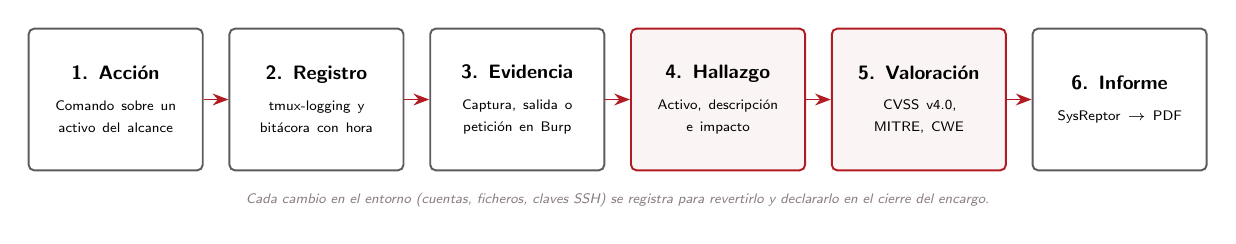
\begin{tikzpicture}[
    font=\sffamily\scriptsize,
    paso/.style={draw=tinta!70, line width=0.7pt, fill=fondo, rounded corners=2pt,
                 text width=2.0cm, minimum height=1.8cm, align=center, inner sep=3pt},
    pasoac/.style={paso, fill=zona, draw=acento},
    flecha/.style={-{Stealth[length=2mm]}, line width=0.7pt, draw=acento}
  ]
  \node[paso]   (p1) at (0,0)     {\textbf{1. Acción}\\[3pt]{\tiny Comando sobre un activo del alcance}};
  \node[paso]   (p2) at (2.55,0)  {\textbf{2. Registro}\\[3pt]{\tiny tmux-logging y bitácora con hora}};
  \node[paso]   (p3) at (5.1,0)   {\textbf{3. Evidencia}\\[3pt]{\tiny Captura, salida o petición en Burp}};
  \node[pasoac] (p4) at (7.65,0)  {\textbf{4. Hallazgo}\\[3pt]{\tiny Activo, descripción e impacto}};
  \node[pasoac] (p5) at (10.2,0)  {\textbf{5. Valoración}\\[3pt]{\tiny CVSS v4.0, MITRE, CWE}};
  \node[paso]   (p6) at (12.75,0) {\textbf{6. Informe}\\[3pt]{\tiny SysReptor $\rightarrow$ PDF}};
  \foreach \a/\b in {p1/p2,p2/p3,p3/p4,p4/p5,p5/p6} \draw[flecha] (\a) -- (\b);
  \node[font=\sffamily\tiny\itshape, text=guia, anchor=north] at ($(p1.south)!0.5!(p6.south)+(0,-0.15)$)
    {Cada cambio en el entorno (cuentas, ficheros, claves SSH) se registra para revertirlo y declararlo en el cierre del encargo.};
\end{tikzpicture}
\caption{Flujo de trabajo desde la acción hasta el informe}
\label{fig:flujo-evidencia}
\end{figure}

\subsection{Herramientas empleadas}

La Tabla~\ref{tab:herramientas} recoge las principales herramientas utilizadas, todas de uso libre o con versión gratuita, y su función en la prueba.

\begin{table}[H]
  \centering
  \caption{Herramientas empleadas en la prueba}
  \label{tab:herramientas}
  \footnotesize
  \estilotabla[1.5]
  \begin{tabularx}{\linewidth}{P{0.7} P{1.3}}
    \reglasup
    \rowcolor{cabecera}
    \cab{Herramienta} & \cab{Función en la prueba} \\
    \rowcolor{filaalterna}
    \textbf{Nmap} & Descubrimiento de hosts y puertos, detección de versiones y \emph{scripts} NSE de enumeración. \\
    \textbf{dig, ffuf y Gobuster} & Transferencia de zona DNS, \emph{fuzzing} de \emph{vhosts} y descubrimiento de directorios y ficheros. \\
    \rowcolor{filaalterna}
    \textbf{Burp Suite Community} & Proxy de intercepción para el análisis manual de las aplicaciones web. \\
    \textbf{EyeWitness, WPScan y sqlmap} & Capturas de los \emph{vhosts}, auditoría de WordPress y verificación de inyecciones SQL. \\
    \rowcolor{filaalterna}
    \textbf{Metasploit Framework} & Explotación y gestión de sesiones cuando aporta frente a la explotación manual. \\
    \textbf{Ligolo-ng, Chisel y SSH} & \emph{Pivoting} y túneles hacia las redes internas; \emph{proxychains} para encaminar herramientas. \\
    \rowcolor{filaalterna}
    \textbf{BloodHound CE} & Recolección (SharpHound / bloodhound-python) y análisis de rutas de ataque en Active Directory. \\
    \textbf{Impacket, NetExec, Responder, Rubeus y Mimikatz} & Enumeración y ataques a protocolos y credenciales de Windows y Active Directory. \\
    \rowcolor{filaalterna}
    \textbf{hashcat y John the Ripper} & Auditoría de contraseñas sobre los \emph{hashes} obtenidos. \\
    \textbf{Obsidian y tmux-logging} & Base de conocimiento de la prueba y registro íntegro de la terminal. \\
    \reglainf
  \end{tabularx}
\end{table}

% ============================ 3 =====================================
\chapter{Desarrollo de la prueba}
\label{cap:desarrollo}

Este capítulo narra la cadena de ataque fase a fase. Para cada fase se indica el objetivo, la metodología seguida, las herramientas empleadas y la técnica de MITRE ATT\&CK asociada, y se dejan los huecos para las evidencias (capturas de pantalla). Los comandos que se muestran son \textbf{ilustrativos} de la técnica empleada; los valores concretos de cada ejecución (direcciones, nombres de \emph{host}, usuarios y credenciales descubiertos) se recogen, enmascarados, en los anexos.

% ---------------------------------------------------------------------
\section{Reconocimiento externo}
\label{sec:recon}

\textbf{Objetivo.} Inventariar la superficie de ataque visible desde Internet sin interactuar aún con las aplicaciones: hosts activos, puertos, servicios, versiones y, sobre todo, los subdominios de \texttt{inlanefreight.local}. \emph{Técnicas MITRE ATT\&CK: T1595 (Active Scanning), T1590 (Gather Victim Network Information), T1590.002 (DNS).}

\textbf{Metodología.} Se comenzó con un barrido completo de puertos sobre el host perimetral y, a continuación, una detección de versiones y \emph{scripts} de enumeración sobre los puertos abiertos. El servicio DNS expuesto se comprobó frente a una \textbf{transferencia de zona}, que, cuando está mal configurada, revela de una sola vez todos los registros del dominio, incluidos los subdominios internos. Los nombres obtenidos se añadieron al fichero \texttt{/etc/hosts} del equipo auditor para poder resolverlos, y la superficie web se amplió con \emph{fuzzing} de \emph{virtual hosts}.

\begin{consola}
# Barrido completo de puertos y, después, versiones sobre los abiertos
nmap -p- --min-rate 2000 -oA nmap/dmz-full 10.129.x.x
nmap -sC -sV -p <puertos_abiertos> -oA nmap/dmz-serv 10.129.x.x

# Comprobacion de transferencia de zona DNS
dig axfr inlanefreight.local @10.129.x.x

# Fuzzing de virtual hosts sobre el servicio web
ffuf -w /usr/share/seclists/Discovery/DNS/subdomains-top1million-5000.txt \
     -u http://10.129.x.x -H "Host: FUZZ.inlanefreight.local" -fs <tamano_base>
\end{consola}

\textbf{Resultado.} \guia{Resume aquí tu resultado real: qué puertos y servicios expuestos encontraste, si la transferencia de zona tuvo éxito y qué subdominios y vhosts identificaste. No incluyas la IP completa ni las flags.}

\imagen{capturas/01_nmap.png}{Resultado del escaneo de puertos y servicios del host perimetral}{fig:nmap}
\imagen{capturas/02_dns_vhosts.png}{Enumeración de DNS y descubrimiento de subdominios}{fig:dns}

% ---------------------------------------------------------------------
\section{Enumeración de servicios}
\label{sec:enum-serv}

\textbf{Objetivo.} Caracterizar cada servicio expuesto del perímetro (FTP, SSH, SMTP/POP3, DNS y HTTP/S) para identificar configuraciones débiles, usuarios válidos y vías potenciales de acceso. \emph{Técnicas MITRE ATT\&CK: T1046 (Network Service Discovery), T1589 (Gather Victim Identity Information).}

\textbf{Metodología.} Para cada servicio se verificaron banners y versiones, se comprobó la existencia de accesos anónimos o por defecto y se enumeraron usuarios cuando el protocolo lo permitía (por ejemplo, mediante los comandos \texttt{VRFY}/\texttt{EXPN} o \texttt{RCPT} en el servicio de correo). El objetivo en esta fase no es explotar, sino construir un inventario preciso que oriente las fases siguientes.

\textbf{Resultado.} \guia{Indica qué servicios resultaron relevantes, si alguno permitía acceso anónimo o enumeración de usuarios, y qué información reutilizaste después (por ejemplo, una lista de usuarios válidos).}

\imagen{capturas/03_enum_servicios.png}{Enumeración de los servicios expuestos en el perímetro}{fig:enum-serv}

% ---------------------------------------------------------------------
\section{Enumeración y explotación web}
\label{sec:web}

\textbf{Objetivo.} Analizar cada aplicación web de los subdominios descubiertos e identificar vulnerabilidades explotables que permitan obtener información sensible o la ejecución de código. \emph{Técnicas MITRE ATT\&CK: T1190 (Exploit Public-Facing Application), T1505.003 (Web Shell); referencia OWASP WSTG.}

\textbf{Metodología.} Cada \emph{vhost} se revisó de forma sistemática siguiendo la OWASP WSTG: mapeo con Burp Suite, descubrimiento de contenido con \emph{fuzzing} de directorios, identificación de la tecnología (CMS, \emph{frameworks}, versiones) y auditoría dirigida de las entradas. Se prestó especial atención a las categorías de mayor impacto: inyección SQL, inclusión de ficheros (LFI/RFI), subida de ficheros sin validar, inyección de comandos y componentes desactualizados con vulnerabilidades conocidas. Cada hallazgo se confirmó con una \textbf{prueba de concepto controlada}, sin acciones destructivas.

\begin{consola}
# Captura e inventario de los vhosts descubiertos
eyewitness --web -f vhosts.txt -d informe/eyewitness

# Descubrimiento de contenido por vhost
feroxbuster -u http://app.inlanefreight.local -w /usr/share/seclists/Discovery/Web-Content/raft-medium-directories.txt

# Auditoria de un WordPress, si procede
wpscan --url http://blog.inlanefreight.local --enumerate vp,u
\end{consola}

\textbf{Resultado.} \guia{Documenta, por cada aplicación vulnerable: la URL (subdominio), el tipo de vulnerabilidad, la prueba de concepto y qué permitió obtener (credenciales, lectura de ficheros, ejecución de código). Enlaza cada una con su hallazgo del capítulo 4. Enmascara credenciales y no incluyas payloads completos que no sean necesarios para entender el hallazgo.}

\imagen{capturas/04_web_hallazgo.png}{Prueba de concepto de la vulnerabilidad web principal}{fig:web}

% ---------------------------------------------------------------------
\section{Acceso inicial al perímetro}
\label{sec:acceso}

\textbf{Objetivo.} Convertir la explotación web en un acceso interactivo y estable al servidor perimetral. \emph{Técnicas MITRE ATT\&CK: T1190 $\rightarrow$ T1059 (Command and Scripting Interpreter), T1078 (Valid Accounts).}

\textbf{Metodología.} A partir de la vulnerabilidad web (por ejemplo, una \emph{web shell} subida o credenciales descubiertas reutilizadas en SSH), se obtuvo una \emph{shell} en el servidor. A continuación se \textbf{estabilizó} la sesión (TTY interactiva) para trabajar con comodidad y se verificó la identidad y los privilegios del usuario obtenido. Todo acceso quedó registrado para su posterior reversión.

\begin{consola}
# Estabilizacion de una shell basica (patron habitual)
python3 -c 'import pty; pty.spawn("/bin/bash")'
# (Ctrl-Z) stty raw -echo; fg   ->   export TERM=xterm

# Comprobacion de identidad y privilegios
id && hostname && ip a
\end{consola}

\textbf{Resultado.} \guia{Explica cómo obtuviste el acceso inicial (web shell, credenciales reutilizadas, etc.), con qué usuario y qué nivel de privilegios tenías en ese momento.}

\imagen{capturas/05_acceso_inicial.png}{Obtención del acceso inicial al servidor perimetral}{fig:acceso}

% ---------------------------------------------------------------------
\section{Escalada de privilegios local}
\label{sec:privesc}

\textbf{Objetivo.} Elevar los privilegios en el servidor comprometido hasta \texttt{root} (Linux) o \texttt{SYSTEM} (Windows). \emph{Técnicas MITRE ATT\&CK: T1068 (Exploitation for Privilege Escalation), T1548 (Abuse Elevation Control Mechanism).}

\textbf{Metodología.} Se ejecutaron herramientas de enumeración local (\texttt{linPEAS} / \texttt{winPEAS}) para identificar vías de escalada: permisos \texttt{sudo} mal configurados, binarios SUID, tareas programadas, servicios con permisos débiles, credenciales almacenadas en ficheros o versiones de \emph{kernel} vulnerables. La vía elegida se ejecutó de forma controlada y reversible.

\textbf{Resultado.} \guia{Indica la vía de escalada concreta que aprovechaste y cómo confirmaste el acceso privilegiado. Relaciónala con el hallazgo correspondiente del capítulo 4.}

\imagen{capturas/06_privesc.png}{Escalada de privilegios local en el servidor comprometido}{fig:privesc}

% ---------------------------------------------------------------------
\section{Persistencia controlada y pivoting}
\label{sec:pivoting}

\textbf{Objetivo.} Establecer un acceso persistente, controlado y reversible, y abrir una vía hacia las redes internas no accesibles desde Internet. \emph{Técnicas MITRE ATT\&CK: T1098 (Account Manipulation), T1090 (Proxy), T1572 (Protocol Tunneling), T1046 (Network Service Discovery).}

\textbf{Metodología.} Tras documentar el acceso privilegiado, se identificaron las interfaces internas del servidor (doble \emph{homing} hacia \texttt{172.16.8.0/23}). Se levantó un túnel con \textbf{Ligolo-ng} (o Chisel como alternativa) para encaminar el tráfico del equipo auditor hacia la red interna, y desde ahí se enumeraron hosts y servicios internos. Toda persistencia creada (claves SSH, cuentas o servicios) se anotó para revertirla en el cierre.

\begin{consola}
# Pivoting con Ligolo-ng (patron habitual)
# En el equipo auditor (proxy/relay):
./proxy -selfcert
# En el host comprometido (agente):
./agent -connect <ip_auditor>:11601 -ignore-cert

# Reconocimiento de la red interna a traves del tunel
nmap -sn 172.16.8.0/23          # hosts activos
nmap -sT -p 88,139,389,445,3389,5985 172.16.8.0/23
\end{consola}

\textbf{Resultado.} \guia{Describe la red interna descubierta (hosts, roles aparentes y servicios de dominio como LDAP/Kerberos/SMB) y confirma que el pivoting funcionaba. Lista en el Anexo los artefactos de persistencia creados y su reversión.}

\imagen{capturas/07_pivoting.png}{Túnel hacia la red interna y reconocimiento de hosts}{fig:pivoting}

% ---------------------------------------------------------------------
\section{Enumeración de Active Directory}
\label{sec:ad-enum}

\textbf{Objetivo.} Cartografiar el dominio \texttt{INLANEFREIGHT.LOCAL}: usuarios, grupos, equipos, sesiones, relaciones de confianza, ACL y rutas de ataque hacia los administradores de dominio. \emph{Técnicas MITRE ATT\&CK: T1087 (Account Discovery), T1018 (Remote System Discovery), T1069 (Permission Groups Discovery), T1482 (Domain Trust Discovery).}

\textbf{Metodología.} Con las primeras credenciales de dominio obtenidas (o incluso sin autenticar, cuando el dominio lo permite), se recolectó la información del directorio con \textbf{BloodHound} (SharpHound o \texttt{bloodhound-python}) y se complementó con \textbf{NetExec} para validar accesos y enumerar recursos compartidos. El análisis del grafo permite identificar los caminos más cortos hacia \emph{Domain Admins} y las malas configuraciones (privilegios excesivos, ACL peligrosas, sesiones de administradores en equipos accesibles).

\begin{consola}
# Recoleccion para BloodHound desde el equipo auditor (via proxychains)
proxychains bloodhound-python -u '<usuario>' -p '<clave>' \
  -d inlanefreight.local -ns 172.16.8.x -c All --zip

# Validacion de accesos y enumeracion con NetExec
proxychains nxc smb 172.16.8.0/23 -u '<usuario>' -p '<clave>' --shares
\end{consola}

\textbf{Resultado.} \guia{Resume la estructura del dominio y, sobre todo, las rutas de ataque que reveló BloodHound (incluye una captura del grafo). Señala las cuentas y grupos clave que utilizaste después.}

\imagen{capturas/08_bloodhound.png}{Rutas de ataque hacia Domain Admins en BloodHound}{fig:bloodhound}

% ---------------------------------------------------------------------
\section{Ataques a credenciales de dominio}
\label{sec:cred}

\textbf{Objetivo.} Obtener credenciales de dominio adicionales que permitan el movimiento lateral y la elevación de privilegios. \emph{Técnicas MITRE ATT\&CK: T1558.003 (Kerberoasting), T1558.004 (AS-REP Roasting), T1110 (Brute Force), T1552.001 (Credentials In Files).}

\textbf{Metodología.} Se solicitaron \emph{tickets} de servicio de las cuentas con SPN (\textbf{Kerberoasting}) y se comprobaron las cuentas sin preautenticación de Kerberos (\textbf{AS-REP Roasting}). Los \emph{hashes} obtenidos se auditaron \emph{fuera de línea} con \texttt{hashcat} y un diccionario, sin bloquear cuentas. Además, se revisaron recursos compartidos y ficheros de configuración en busca de credenciales en claro.

\begin{consola}
# Kerberoasting y AS-REP Roasting con Impacket (via proxychains)
proxychains GetUserSPNs.py -request -dc-ip 172.16.8.x inlanefreight.local/'<usuario>':'<clave>'
proxychains GetNPUsers.py -request -dc-ip 172.16.8.x inlanefreight.local/ -usersfile usuarios.txt

# Auditoria offline de los hashes obtenidos
hashcat -m 13100 kerberoast.hash /usr/share/wordlists/rockyou.txt   # TGS-REP
hashcat -m 18200 asrep.hash /usr/share/wordlists/rockyou.txt         # AS-REP
\end{consola}

\textbf{Resultado.} \guia{Indica qué cuentas resultaron vulnerables (sin nombrar la contraseña real: enmascárala) y qué privilegios te otorgaron. Relaciona con el hallazgo de contraseñas débiles del capítulo 4.}

\imagen{capturas/09_kerberoasting.png}{Obtención y auditoría de credenciales de servicio}{fig:cred}

% ---------------------------------------------------------------------
\section{Movimiento lateral}
\label{sec:lateral}

\textbf{Objetivo.} Utilizar las credenciales obtenidas para acceder a otros equipos del dominio y acercarse al controlador de dominio. \emph{Técnicas MITRE ATT\&CK: T1021.001 (RDP), T1021.006 (WinRM), T1550.002 (Pass-the-Hash), T1021.002 (SMB).}

\textbf{Metodología.} Con cada nueva credencial se comprobó, mediante NetExec, en qué equipos concedía acceso y con qué nivel de privilegio. El acceso interactivo se obtuvo con \textbf{evil-winrm} (WinRM) o \textbf{xfreerdp} (RDP), y, cuando solo se disponía del \emph{hash} NTLM, mediante \emph{pass-the-hash}. En cada salto se repitió el ciclo de enumeración local y búsqueda de nuevas credenciales.

\begin{consola}
# Validacion masiva de accesos con un par de credenciales
proxychains nxc smb 172.16.8.0/23 -u '<usuario>' -p '<clave>' -d inlanefreight.local

# Acceso interactivo por WinRM
proxychains evil-winrm -i 172.16.8.x -u '<usuario>' -p '<clave>'
\end{consola}

\textbf{Resultado.} \guia{Describe la secuencia de saltos entre equipos y cómo cada acceso te acercó al dominio. Un esquema de la cadena (host A -> host B -> ...) ayuda a seguir la narrativa.}

\imagen{capturas/10_lateral.png}{Movimiento lateral entre equipos del dominio}{fig:lateral}

% ---------------------------------------------------------------------
\section{Compromiso del dominio}
\label{sec:dominio}

\textbf{Objetivo.} Alcanzar privilegios de administrador de dominio y demostrar el control total sobre \texttt{INLANEFREIGHT.LOCAL}. \emph{Técnicas MITRE ATT\&CK: T1003.006 (DCSync), T1003.001 (LSASS Memory), T1098, T1078.002 (Domain Accounts).}

\textbf{Metodología.} La ruta identificada en BloodHound condujo a una cuenta con privilegios suficientes para realizar un \textbf{DCSync}, es decir, solicitar al controlador de dominio la replicación de los secretos del directorio, incluido el \emph{hash} de la cuenta \texttt{krbtgt} y de los administradores. La extracción se realizó con \textbf{Impacket secretsdump}. Con ello se demostró el compromiso total del dominio, sin necesidad de acciones destructivas.

\begin{consola}
# DCSync: replicacion de secretos del dominio (demostracion de impacto)
proxychains secretsdump.py -just-dc inlanefreight.local/'<usuario_privilegiado>':'<clave>'@172.16.8.x
\end{consola}

\textbf{Resultado.} \guia{Confirma el compromiso del dominio (captura de secretsdump con los hashes enmascarados o del acceso al DC). Este es el hallazgo crítico que cierra la cadena de ataque.}

\imagen{capturas/11_dominio.png}{Compromiso del controlador de dominio (DCSync)}{fig:dominio}

% ---------------------------------------------------------------------
\section{Post-explotación, impacto y cierre}
\label{sec:cierre}

\textbf{Objetivo.} Evaluar el impacto real sobre los datos de la organización y cerrar el encargo revirtiendo los cambios. \emph{Técnicas MITRE ATT\&CK: T1005 (Data from Local System), T1039 (Data from Network Shared Drive).}

\textbf{Metodología.} Con el control del dominio, se verificó —sin exfiltrar ni alterar datos— el alcance de la información accesible (recursos compartidos, bases de datos, carpetas de usuarios) para dimensionar el impacto en el negocio. A continuación se ejecutó el \emph{engagement closeout}: se eliminaron las \emph{web shells}, las cuentas y las claves creadas, se restauraron los ficheros modificados y se dejó constancia en la bitácora de todos los artefactos introducidos y revertidos.

\textbf{Resultado.} \guia{Resume el impacto demostrado (qué datos críticos quedaban al alcance) y confirma que todos los cambios se han revertido. Incluye en el Anexo C el registro de cambios y su reversión.}

\imagen{capturas/12_impacto.png}{Evaluación del impacto sobre los datos de la organización}{fig:impacto}

% ============================ 4 =====================================
\chapter{Hallazgos y recomendaciones}
\label{cap:hallazgos}

\guia{Este capítulo se completa al finalizar la práctica, con los hallazgos reales obtenidos durante la prueba. A continuación se deja la estructura (tablas, bloque de hallazgo y plan de remediación) lista para rellenar.}

\section{Resumen de hallazgos}

\guia{Rellena la tabla con todos los hallazgos, ordenados de mayor a menor severidad: identificador (H-01, H-02\dots), descripción breve, severidad y puntuación CVSS v4.0 (calculada con la calculadora de FIRST). Para la columna de severidad puedes usar las etiquetas de color ya definidas en el documento: \texttt{\textbackslash scrit} (crítica), \texttt{\textbackslash salta} (alta), \texttt{\textbackslash smedia} (media) y \texttt{\textbackslash sbaja} (baja).}

\begin{table}[H]
  \centering
  \caption{Hallazgos priorizados}
  \label{tab:hallazgos}
  \footnotesize
  \estilotabla[1.5]
  \begin{tabularx}{\linewidth}{P{0.5} P{1.9} P{0.7} P{0.9}}
    \reglasup
    \rowcolor{cabecera}
    \cab{ID} & \cab{Hallazgo} & \cab{Severidad} & \cab{CVSS v4.0} \\
    \rowcolor{filaalterna}
    \textbf{H-01} & \guia{descripción breve del hallazgo} & \guia{severidad} & \guia{0.0} \\
    \textbf{H-02} & \guia{descripción breve del hallazgo} & \guia{severidad} & \guia{0.0} \\
    \reglainf
  \end{tabularx}
\end{table}

\section{Detalle de los hallazgos}

\guia{Desarrolla cada hallazgo con la estructura del bloque de ejemplo siguiente y repítela para cada uno: encabezado con severidad, técnica de MITRE ATT\&CK y clasificación CWE; y los apartados Descripción, Activos afectados, Impacto, Evidencia (captura) y Remediación.}

\subsection{H-01 · [título del hallazgo]}
\textbf{Severidad:} \guia{nivel}\quad\textbf{MITRE ATT\&CK:} \guia{Txxxx}\quad\textbf{CWE:} \guia{CWE-xxx}

\textbf{Descripción.} \guia{Qué es la vulnerabilidad, dónde está y cómo se explotó durante la prueba.}

\textbf{Activos afectados.} \guia{Hosts, servicios o aplicaciones afectados.}

\textbf{Impacto.} \guia{Consecuencia para la organización si un atacante la aprovechara.}

\textbf{Remediación.} \guia{Medidas concretas para corregir el hallazgo.}

\imagen{capturas/hallazgo_01.png}{Evidencia del hallazgo H-01}{fig:h01}

\section{Recomendaciones priorizadas}
\label{sec:recomendaciones}

\guia{A partir de los hallazgos, define el plan de remediación por horizonte temporal. Rellena la tabla siguiente.}

\begin{table}[H]
  \centering
  \caption{Plan de remediación por horizonte temporal}
  \label{tab:recomendaciones}
  \footnotesize
  \estilotabla[1.5]
  \begin{tabularx}{\linewidth}{P{0.6} P{1.4}}
    \reglasup
    \rowcolor{cabecera}
    \cab{Plazo} & \cab{Medidas} \\
    \rowcolor{filaalterna}
    \textbf{Corto} & \guia{medidas inmediatas, derivadas de los hallazgos críticos y altos} \\
    \textbf{Medio} & \guia{medidas a medio plazo} \\
    \rowcolor{filaalterna}
    \textbf{Largo} & \guia{medidas estructurales y de mejora continua} \\
    \reglainf
  \end{tabularx}
\end{table}

% ============================ 5 =====================================
\chapter{Conclusiones}

\section{Cumplimiento de los objetivos}
\guia{Valora en qué medida se han cumplido los objetivos específicos OE1 a OE8 del anteproyecto: preparación del entorno y alcance (OE1), reconocimiento externo y enumeración (OE2), identificación y explotación de vulnerabilidades web (OE3), acceso inicial y persistencia (OE4), pivoting y compromiso del dominio (OE5), repetición autónoma sin walkthrough (OE6), valoración con CVSS v4.0 y MITRE y propuesta de remediación (OE7), y elaboración del informe, la memoria y el manual (OE8).}

\section{Valoración global}

La prueba confirma la hipótesis de partida del encargo: un atacante externo, sin información previa, puede alcanzar el control total de un dominio de Active Directory encadenando debilidades individualmente moderadas. El valor del ejercicio no reside únicamente en demostrar el compromiso, sino en \textbf{documentarlo de forma reproducible} y en traducirlo a un plan de remediación comprensible y accionable para el cliente. La vertiente defensiva —qué corregir y en qué orden— es tan importante como la ofensiva.

\section{Limitaciones}
\guia{Reflexiona sobre las limitaciones: entorno de laboratorio frente a una red real, ausencia de evasión de AV/EDR en el escenario, alcance acotado por las reglas de enfrentamiento y dependencia de la plataforma de HTB Academy.}

\section{Líneas de mejora}
\guia{Propón cómo continuar: ampliar la prueba con evasión de defensas, automatizar parte de la enumeración, repetir el ejercicio sobre otros módulos del itinerario o contrastar los hallazgos frente a un entorno defensivo (Blue Team) para medir la detección.}

% ===================== DECLARACIÓN DE USO DE IA ======================
\chapter*{Declaración de uso de IA generativa}
\addcontentsline{toc}{chapter}{Declaración de uso de IA generativa}
\markboth{Declaración de uso de IA generativa}{}

En cumplimiento de las normas del proyecto, se declara el uso de la herramienta de inteligencia artificial generativa \textbf{Claude} (Anthropic) como apoyo en la elaboración de este documento. La Tabla~\ref{tab:declaracion-ia} detalla en qué partes y de qué forma se ha utilizado.

\begin{table}[H]
  \centering
  \caption{Uso de IA generativa en la elaboración del trabajo}
  \label{tab:declaracion-ia}
  \small
  \estilotabla
  \begin{tabularx}{\linewidth}{K Y}
    \reglasup
    \rowcolor{cabecera}
    \cab{Parte del trabajo} & \cab{Uso de la IA} \\
    \rowcolor{filaalterna}
    \textbf{Plantilla LaTeX y diseño} & Adaptación de la plantilla, paleta de color y portada al informe técnico \\
    \textbf{Diagramas} & Elaboración de los diagramas de la topología y del flujo de evidencias \\
    \rowcolor{filaalterna}
    \textbf{Estructura del informe} & Organización de capítulos, tablas y marco metodológico \\
    \textbf{Redacción} & Apoyo en la redacción de la narrativa metodológica y las recomendaciones \\
    \reglainf
  \end{tabularx}
\end{table}

La \textbf{parte técnica del proyecto ha sido desarrollada completamente por el alumno}: la ejecución de la prueba de penetración, la obtención de las evidencias, la valoración de los hallazgos y las decisiones de remediación. Todo el contenido generado con ayuda de la IA ha sido revisado y adaptado por el alumno, y las referencias se han contrastado con sus fuentes originales.

% ============================ REFERENCIAS ============================
\chapter{Referencias bibliográficas}

\begin{list}{}{\leftmargin=1.27cm \itemindent=-1.27cm \itemsep=6pt}
  \item FIRST. (2023). \textit{Common Vulnerability Scoring System version 4.0: Specification document}. Forum of Incident Response and Security Teams. \url{https://www.first.org/cvss/v4.0/specification-document}
  \item Hack The Box. (s.~f.). \textit{Attacking Enterprise Networks} [Módulo de HTB Academy]. \url{https://academy.hackthebox.com/course/preview/attacking-enterprise-networks}
  \item Hack The Box. (s.~f.). \textit{HTB Certified Penetration Testing Specialist (HTB CPTS)}. \url{https://academy.hackthebox.com/preview/certifications/htb-certified-penetration-testing-specialist}
  \item Ley Orgánica 10/1995, de 23 de noviembre, del Código Penal. (1995). \textit{Boletín Oficial del Estado}, 281. \url{https://www.boe.es/buscar/act.php?id=BOE-A-1995-25444}
  \item MITRE Corporation. (s.~f.). \textit{MITRE ATT\&CK}. \url{https://attack.mitre.org}
  \item OWASP Foundation. (2020). \textit{Web Security Testing Guide v4.2}. \url{https://owasp.org/www-project-web-security-testing-guide/}
  \item PTES. (s.~f.). \textit{The Penetration Testing Execution Standard}. \url{http://www.pentest-standard.org}
  \item Real Decreto 479/2020, de 7 de abril, por el que se establece el Curso de especialización en ciberseguridad en entornos de las tecnologías de la información. (2020). \textit{Boletín Oficial del Estado}, 134. \url{https://www.boe.es/boe/dias/2020/05/13/pdfs/BOE-A-2020-4962.pdf}
  \item Scarfone, K., Souppaya, M., Cody, A., y Orebaugh, A. (2008). \textit{Technical guide to information security testing and assessment} (NIST SP 800-115). National Institute of Standards and Technology. \url{https://csrc.nist.gov/pubs/sp/800/115/final}
\end{list}

\guia{Añade en formato APA 7.ª edición las fuentes adicionales que cites (por ejemplo, la documentación de las herramientas concretas que utilices) y mantén el orden alfabético.}

% ============================ ANEXOS ================================
\appendix
\renewcommand{\appendixname}{Anexo}

\chapter{Inventario de hosts y servicios}
\guia{Tabla con los hosts descubiertos (externos e internos), su sistema operativo aparente, los servicios relevantes y su papel en la cadena de ataque. No incluyas la IP externa completa del laboratorio.}

\chapter{Credenciales comprometidas (enmascaradas)}
\guia{Relación de las credenciales obtenidas durante la prueba, con la contraseña enmascarada (por ejemplo, Pa\$\$...\ o solo los 3 primeros caracteres). Indica el origen de cada una y los accesos que concedía. No publiques credenciales ni flags en claro.}

\begin{table}[H]
  \centering
  \caption{Credenciales comprometidas (valores enmascarados)}
  \label{tab:credenciales}
  \footnotesize
  \estilotabla[1.5]
  \begin{tabularx}{\linewidth}{P{1.0} P{0.7} P{1.3} P{1.0}}
    \reglasup
    \rowcolor{cabecera}
    \cab{Usuario} & \cab{Tipo} & \cab{Origen} & \cab{Acceso que concede} \\
    \rowcolor{filaalterna}
    \guia{usuario1} & \guia{clave/hash} & \guia{web / Kerberoasting / ...} & \guia{host o rol} \\
    \guia{usuario2} & \guia{clave/hash} & \guia{...} & \guia{...} \\
    \reglainf
  \end{tabularx}
\end{table}

\chapter{Registro de cambios en el entorno y su reversión}
\guia{Lista de todos los artefactos introducidos durante la prueba (web shells, cuentas, claves SSH, ficheros) con la fecha, el host y la acción de reversión aplicada en el cierre del encargo. Es la evidencia de que el entorno quedó limpio.}

\chapter{Relación con los resultados de aprendizaje}

La Tabla~\ref{tab:ra} relaciona el trabajo con los resultados de aprendizaje del módulo de Hacking Ético.

\begin{table}[H]
  \centering
  \caption{Aportación del proyecto a los resultados de aprendizaje}
  \label{tab:ra}
  \footnotesize
  \estilotabla[1.5]
  \begin{tabularx}{\linewidth}{P{0.95} P{1.05}}
    \reglasup
    \rowcolor{cabecera}
    \cab{Resultado de aprendizaje} & \cab{Aportación del proyecto} \\
    \rowcolor{filaalterna}
    \textbf{RA1.} Determina herramientas de monitorización para detectar vulnerabilidades aplicando técnicas de hacking ético. & Fases del hacking ético aplicadas a un encargo completo, con permisos previos, reconocimiento y documentación de vulnerabilidades con CVSS v4.0. \\
    \textbf{RA3.} Ataca y defiende en entornos de prueba, redes y sistemas consiguiendo acceso a información y sistemas de terceros. & Reconocimiento, explotación de servicios, escalada en Linux y Windows y ataques a Active Directory hasta el compromiso del dominio. \\
    \rowcolor{filaalterna}
    \textbf{RA4.} Consolida y utiliza sistemas comprometidos garantizando accesos futuros. & Persistencia controlada en la DMZ, pivoting hacia la red interna, administración remota (SSH, WinRM, RDP) y auditoría de contraseñas sobre los hashes obtenidos. \\
    \textbf{RA5.} Ataca y defiende en entornos de prueba, aplicaciones web consiguiendo acceso a datos o funcionalidades no autorizadas. & Análisis con proxy de intercepción y explotación de los subdominios web de Inlanefreight; cada hallazgo incluye su remediación (vertiente defensiva). \\
    \reglainf
  \end{tabularx}
\end{table}

\guia{Ajusta los resultados de aprendizaje a los definidos en tu módulo de Hacking Ético si difieren de estos.}

\end{document}